% Figure M9 hero prototype : generated by experiments/m9_scrna.py --hero.
% Preview-only; not yet linked from the main manuscript.
\begin{figure}[t]
 \centering
 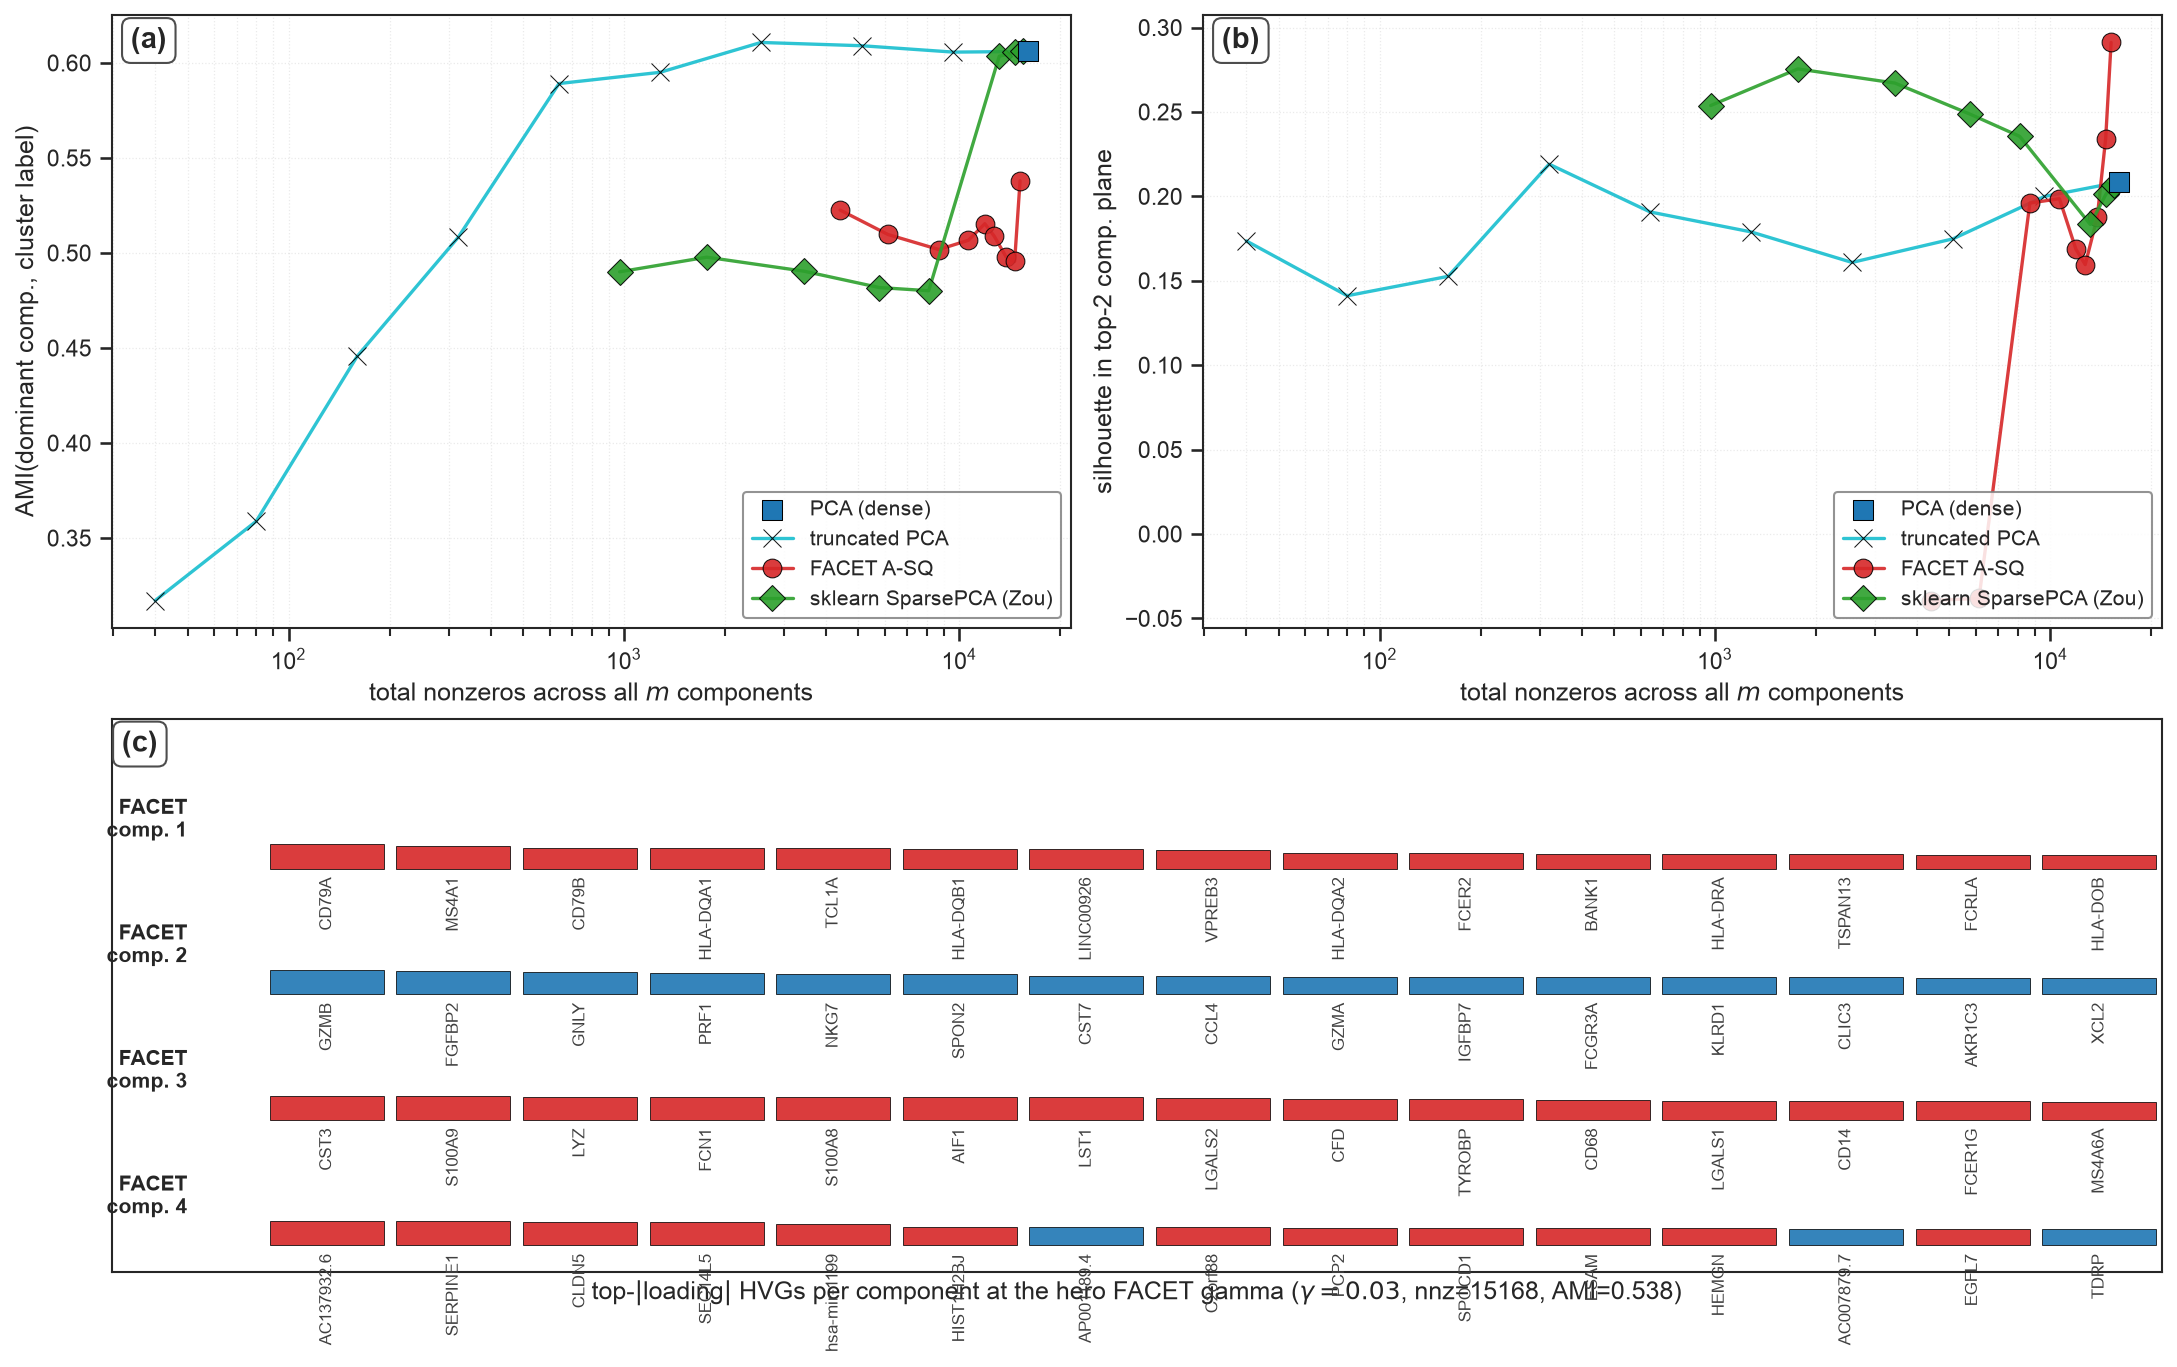
\includegraphics[width=\linewidth]{../shared/figures/generated/m9_scrna_hero.png}
 \caption{\textbf{M9: single-cell RNA-seq on 10x Genomics PBMC 3k, matched-sparsity sweep.} 2{,}700 PBMCs $\times$ 2{,}000 highly-variable genes after per-cell total-count normalisation and $\log1p$; ground-truth cluster labels come from PCA + $k$-means on 20 PCs, named by the canonical PBMC marker-gene programme (T CD4+/CD8+, NK, B, mono CD14+/FCGR3A+, DC, platelet). \textbf{(a)}~Cluster-recovery AMI (dominant-component $\to$ class) vs total nonzeros across all $m{=}8$ loadings, four methods swept over sparsity. Dense PCA (blue square) sets the ceiling at AMI $0.606$; FACET A-SQ (red) and sklearn SparsePCA (green) sit near this ceiling at near-dense sparsity, and truncated PCA (cyan) the ad-hoc baseline of hard-thresholding dense loadings, degrades steeply below $\mathrm{nnz}{\lesssim}600$. \textbf{(b)}~Silhouette in the top-two variance-dominant component plane. FACET A-SQ attains the highest silhouette of any method ($0.291$ at $\gamma{=}0.03$) exceeding dense PCA ($0.208$) SparsePCA's best ($0.276$) and every truncated-PCA cell. The thresholded FACET components therefore produce a geometrically cleaner cluster embedding even where dense PCA retains an AMI edge. \textbf{(c)}~Top-15 gene loadings per component for FACET at the hero $\gamma$. Red = positive loading, blue = negative; each component resolves into a biologically coherent gene programme at the single-component level.}
 \label{fig:m9-scrna-hero}
\end{figure}
